% Document class and two-column conversion
\documentclass[twocolumn]{report}
% dimensions of paper and relative text positioning
\usepackage[a4paper,top=2cm,bottom=2cm,left=2cm,right=2cm]{geometry}
% package for including URLs
\usepackage{url}
% Required for including images
\usepackage{graphicx}

\setlength{\parindent}{0pt} % Removes all indentation from paragraphs

% Start of the document
\begin{document}

% Title page
\title{\Huge \bfseries Optimization techniques: First Assignment} %\Huge and \bfseries are used to make the title bigger and bold
\author{Konstantinos Fotios Papadakis\vspace{0.5cm} \\  AEM:10371} % \vspace{0.5cm} is used to add some vertical space between the author and the AEM
\date{\today}
% prints the title, author and date on a separate page
\maketitle

% Table of contents page
\tableofcontents

% Dichotomy
\chapter{Problem 1}
\section{Prompt}
Υλοποιήστε στο \selectlanguage{english}Matlab \selectlanguage{greek} τη μέθοδο της Διχοτόμου και εφαρμόστε τη στις 
συναρτήσεις $f_1(x)$, $f_2(x)$, $f_3(x)$.
\begin{itemize}
    \item Κρατώντας σταθερό το τελικό εύρος αναζήτησης $l = 0.01$ μελετήστε τη μεταβολή των
υπολογισμών της αντικειμενικής συνάρτησης $f_i(x)$, $i = 1,2,3$ (δηλαδή τον συνολικό αριθμό που
χρειάστηκε να υπολογιστεί η $f(x)$, για τις δεδομένες τιμές των $l$ και $\epsilon$, μέχρι να τερματίσει ο
αλγόριθμος), καθώς μεταβάλλουμε τη σταθερά $\epsilon > 0$ (απόσταση από τη διχοτόμο).
Δημιουργήστε τις αντίστοιχες γραφικές παραστάσεις από τις τιμές που προκύπτουν για τις τρεις
συναρτήσεις.
    \item Κρατώντας σταθερό το $\epsilon = 0.001$ μελετήστε τη μεταβολή των υπολογισμών της $f_i(x)$, 
$i=1,2,3$, καθώς μεταβάλλουμε το $l$. Δημιουργήστε τις αντίστοιχες γραφικές παραστάσεις από τις
τιμές που προκύπτουν για τις τρεις συναρτήσεις.
    \item Επιπλέον, σε τρία διαγράμματα, ένα για κάθε συνάρτηση, σχεδιάστε τις γραφικές παραστάσεις
των άκρων του διαστήματος $[a_k, b_k]$ συναρτήσει του δείκτη επαναλήψεων $k$, δηλαδή $(k, a_k)$ και
$(k, b_k)$, για διάφορες τιμές του τελικού εύρους αναζήτησης $l$.
\end{itemize}
\section{Solution}
Κατανόηση Αλγορίθμου

Χωρίζουμε το αρχικό μας χωρίο σε τρία ανισομερή υπό-διαστήματα χρησιμοποιώντας τα σημεία $x1$ και $x2$.
To determine the correct subinterval to commence our new search we use the Θεώρημα 5.1.1 του βιβλίου.
Σύμφωνα με αυτό, αν μια συνάρτηση $f$ είναι \textbf{αυστηρά σχεδόν κυρτή} σε ένα διάστημα $[a,b]$
όπου $x_1,x_2 \epsilon[a,b]$ και $a < x_1 < x_2 < b$, τότε αν $f(x_1)<f(x_2)$, $f(x)>=f(x_1)$ για κάθε
$x \epsilon [x_2,b]$. Ομοίως, αν $f(x_1)>=f(x_2)$, $f(x)>=f(x_2)$ για κάθε $x \epsilon [a,x_1]$.

Βήματα Αλγορίθμου:
\begin{enumerate}
    \item Ελέγχουμε αν $b - a < l$. Αν ισχύει, σταματάμε την αναζήτηση.
    \item Στην περίπτωση που δεν ισχύει, θέτουμε $x1=\frac{a+b}{2}-\epsilon$ και
    $x2=\frac{a+b}{2}+\epsilon$.
    \item Αν $f(x_1) < f(x_2)$, θέτουμε $a_{k+1}=a_k$ και $b_{k+1}=x_{2k}$.
    \item Αλλιώς θέτουμε $a_(k+1)=x_(1k)$ και $b_(k+1)=b_k$.
    \item Μεταβαίνουμε στην επόμενη επανάληψη του αλγορίθμου $k=k+1$ και σταματάμε όταν
    $b_k - a_k < l$.
\end{enumerate}

% Golden section 
\chapter{Problem 2}
\section{Prompt}
Υλοποιήστε στο \selectlanguage{english}Matlab \selectlanguage{greek} τη μέθοδο του Χρυσού Τομέα και 
εφαρμόστε τη στις συναρτήσεις $f_1(x)$, $f_2(x)$, $f_3(x)$.
\begin{itemize}
    \item Μελετήστε τη μεταβολή των υπολογισμών της αντικειμενικής συνάρτησης $f_i(x)$, $i = 1,2,3$
    (δηλαδή τον συνολικό αριθμό που πρέπει να υπολογιστεί η $f_i(x)$ μέχρι να τερματίσει ο
    αλγόριθμος), καθώς μεταβάλλουμε το τελικό εύρος αναζήτησης $l$. Δημιουργήστε τις αντίστοιχες
    γραφικές παραστάσεις από τις τιμές που προκύπτουν για τις τρεις συναρτήσεις.

    \item Επιπλέον, σε τρία διαγράμματα, ένα για κάθε συνάρτηση, σχεδιάστε τις γραφικές παραστάσεις
    των άκρων του διαστήματος $[a_k, b_k]$ συναρτήσει του δείκτη επαναλήψεων $k$, δηλαδή
    $(k, a_k)$ και $(k, b_k)$, για διάφορες τιμές του τελικού εύρους αναζήτησης $l$.
\end{itemize}
\section{Solution}
\subsection{Κατανόηση Αλγορίθμου}
Η μέθοδος του χρυσού τομέα διαμορφώνει διαστήματα αναζήτησης τα οποία είναι αναλογικά μεταξύ τους.
Συγκεκριμένα ο λόγος μεταξύ δύο διαδοχικών χωρίων είναι ίσος με την σταθερά γ. Ένα κομμάτι στο 
οποίο η μέθοδος αυτή βελτιώνει την μέθοδο της διχοτόμησης είναι ότι μετά την πρώτη φορά που
υπολογίζει τις τιμές της συνάρτησης τις επόμενες επαναλήψεις χρειάζεται να υπολογίσει μόνο
μία τιμή της συνάρτησης. 

\subsection{Υπολογισμοί αντικειμενικής συνάρτησης συναρτήσει του $l$}

\begin{figure}[H] % h for 'here', you can also use t (top), b (bottom), or p (page)
    \centering
    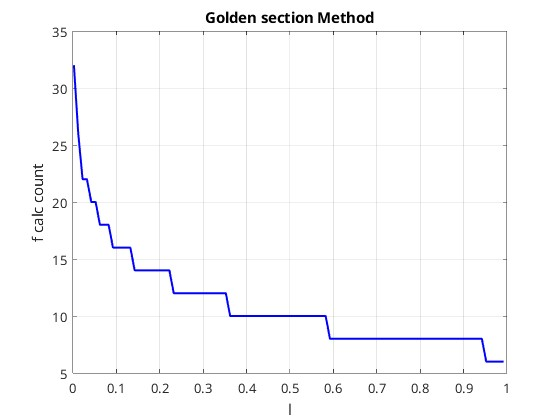
\includegraphics[width=0.5\textwidth]{media/goldenf1} % Image file without extension
    \caption{Συνάρτηση $f_1$}
\end{figure}

\begin{figure}[H] % h for 'here', you can also use t (top), b (bottom), or p (page)
    \centering
    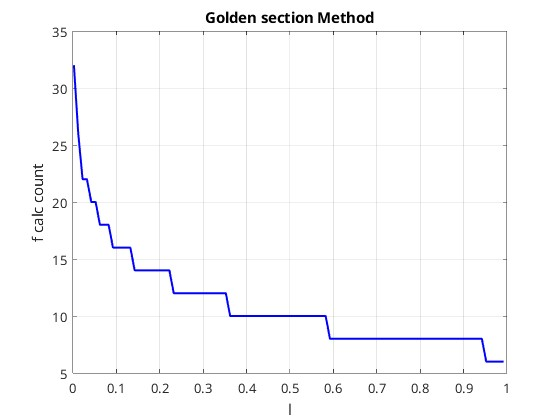
\includegraphics[width=0.5\textwidth]{media/goldenf2} % Image file without extension
    \caption{Συνάρτηση $f_2$}
\end{figure}

\begin{figure}[H] % h for 'here', you can also use t (top), b (bottom), or p (page)
    \centering
    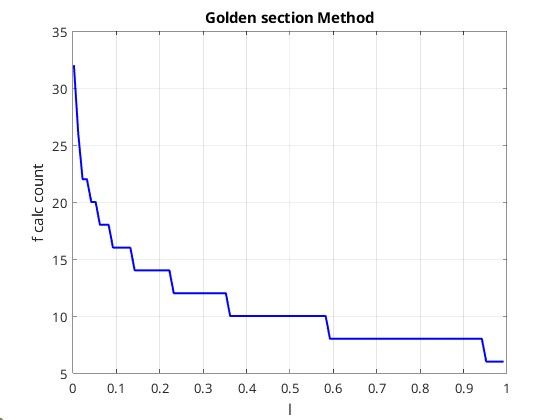
\includegraphics[width=0.5\textwidth]{media/goldenf3} % Image file without extension
    \caption{Συνάρτηση $f_3$}
\end{figure}

\subsection{Άκρα του διαστήματος αναζήτησης συναρτήσει του δείκτη επαναλήψεων}
Συνάρτηση $f_1$:
\begin{figure}[H] % h for 'here', you can also use t (top), b (bottom), or p (page)
    \centering
    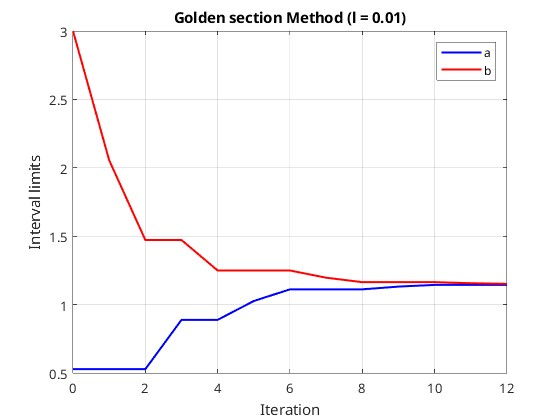
\includegraphics[width=0.5\textwidth]{media/goldenf1_001} % Image file without extension
    \caption{Συνάρτηση $f_1$}
\end{figure}
\begin{figure}[H] % h for 'here', you can also use t (top), b (bottom), or p (page)
    \centering
    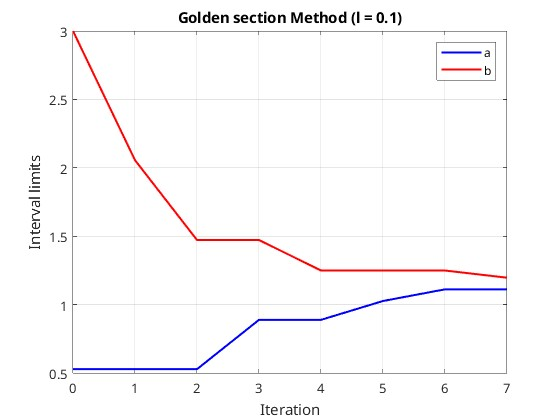
\includegraphics[width=0.5\textwidth]{media/goldenf1_01} % Image file without extension
    \caption{Συνάρτηση $f_1$}
\end{figure}
\begin{figure}[H] % h for 'here', you can also use t (top), b (bottom), or p (page)
    \centering
    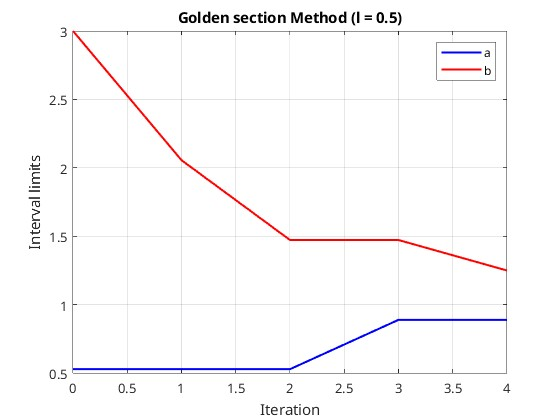
\includegraphics[width=0.5\textwidth]{media/goldenf1_05} % Image file without extension
    \caption{Συνάρτηση $f_1$}
\end{figure}

Συνάρτηση $f_2$:
\begin{figure}[H] % h for 'here', you can also use t (top), b (bottom), or p (page)
    \centering
    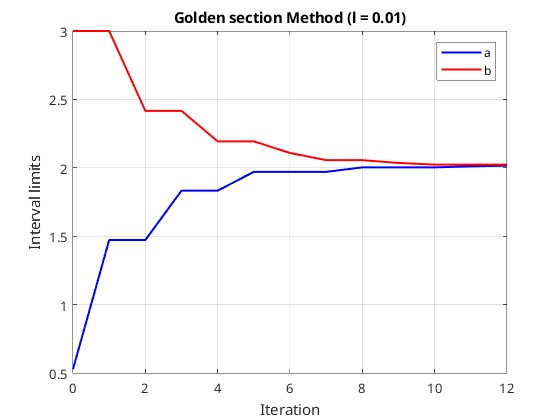
\includegraphics[width=0.5\textwidth]{media/goldenf2_001} % Image file without extension
    \caption{Συνάρτηση $f_2$}
\end{figure}
\begin{figure}[H] % h for 'here', you can also use t (top), b (bottom), or p (page)
    \centering
    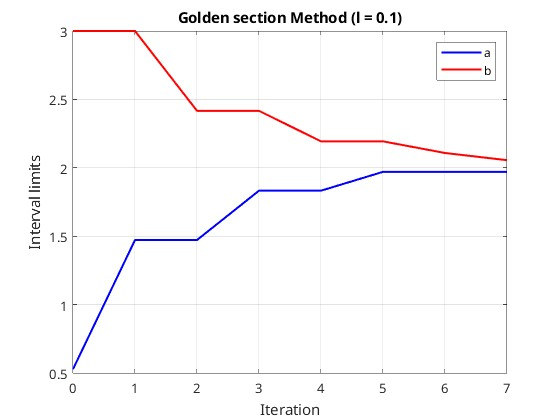
\includegraphics[width=0.5\textwidth]{media/goldenf2_01} % Image file without extension
    \caption{Συνάρτηση $f_2$}
\end{figure}
\begin{figure}[H] % h for 'here', you can also use t (top), b (bottom), or p (page)
    \centering
    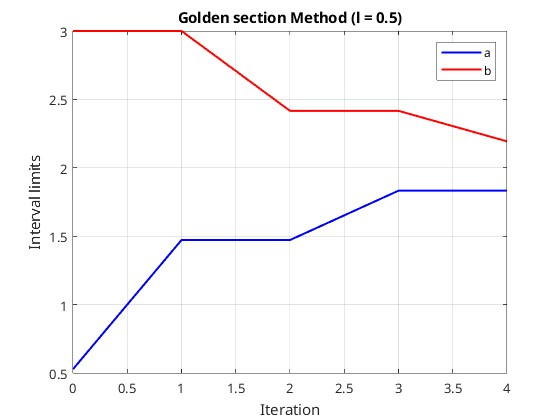
\includegraphics[width=0.5\textwidth]{media/goldenf2_05} % Image file without extension
    \caption{Συνάρτηση $f_2$}
\end{figure}

Συνάρτηση $f_3$:
\begin{figure}[H] % h for 'here', you can also use t (top), b (bottom), or p (page)
    \centering
    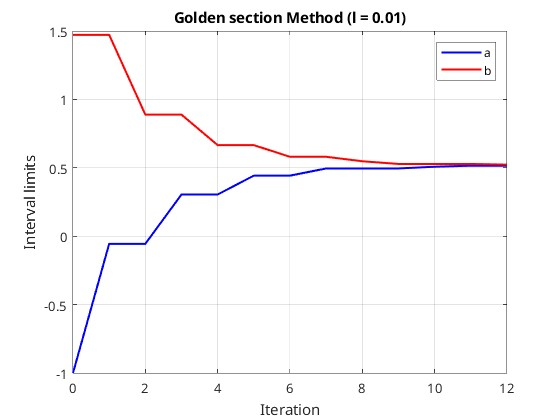
\includegraphics[width=0.5\textwidth]{media/goldenf3_001} % Image file without extension
    \caption{Συνάρτηση $f_3$}
\end{figure}
\begin{figure}[H] % h for 'here', you can also use t (top), b (bottom), or p (page)
    \centering
    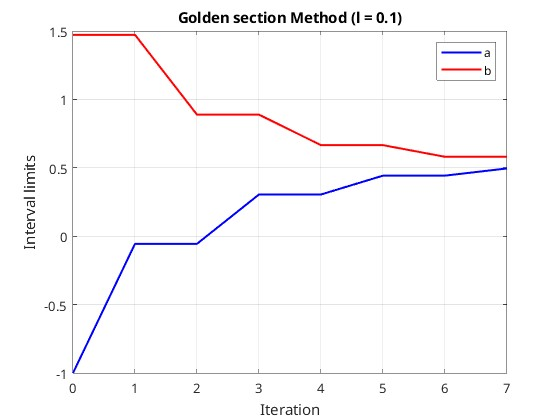
\includegraphics[width=0.5\textwidth]{media/goldenf3_01} % Image file without extension
    \caption{Συνάρτηση $f_3$}
\end{figure}
\begin{figure}[H] % h for 'here', you can also use t (top), b (bottom), or p (page)
    \centering
    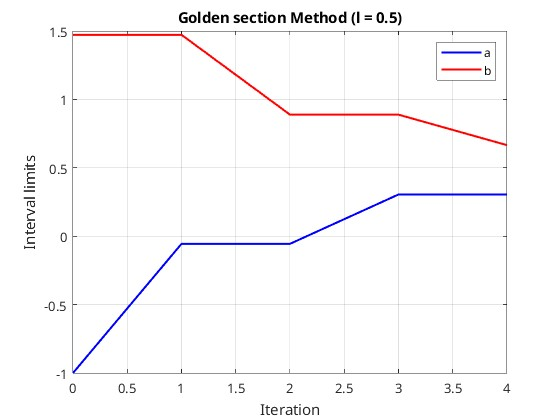
\includegraphics[width=0.5\textwidth]{media/goldenf3_05} % Image file without extension
    \caption{Συνάρτηση $f_3$}
\end{figure}

% FIbonacci 
\chapter{Problem 3}
\section{Prompt}
Επαναλάβετε το Θέμα 2, χρησιμοποιώντας τη μέθοδο \selectlanguage{english}Fibonacci \selectlanguage{greek}.
\section{Solution}
\subsection{Κατανόηση Αλγορίθμου}
Ο αλγόριθμος αυτός βασίζεται στην ακολουθία \selectlanguage{english}Fibonacci\selectlanguage{greek}
μέσω της οποίας ορίζονται διαστήματα αναζήτησης πολύ πιο αποτελεσματικά από τις άλλες μεθόδους. Αυτό 
συμβαίνει επειδή μειώνουμε το διάστημα αναζήτησης κατά $\frac{F_{n-k}}{F_{n-k-1}}$ περισσότερο από όσο
μειωνόταν με τους προηγούμενους αλγορίθμους. Ακόμη, όπως και στον αλγόριθμο της χρυσής τομής εξοικονομούμε
πόρους υπολογίζοντας λιγότερες φορές τις τιμές της εκάστοτε συνάρτησής μας.

\subsection{Υπολογισμοί αντικειμενικής συνάρτησης συναρτήσει του $l$}
\begin{figure}[H] % h for 'here', you can also use t (top), b (bottom), or p (page)
    \centering
    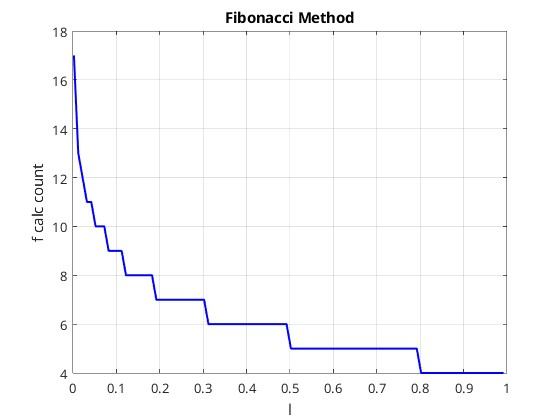
\includegraphics[width=0.5\textwidth]{media/fibonaccif1} % Image file without extension
    \caption{Συνάρτηση $f_1$}
\end{figure}

\begin{figure}[H] % h for 'here', you can also use t (top), b (bottom), or p (page)
    \centering
    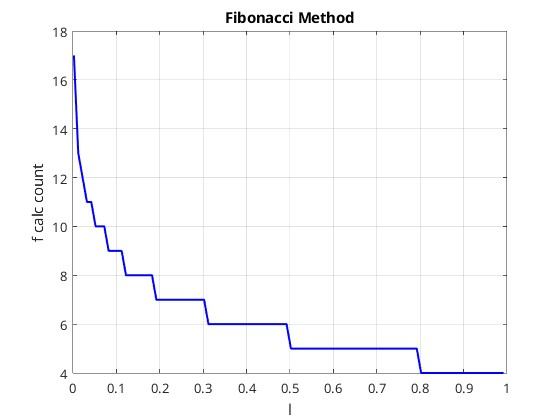
\includegraphics[width=0.5\textwidth]{media/fibonaccif2} % Image file without extension
    \caption{Συνάρτηση $f_2$}
\end{figure}

\begin{figure}[H] % h for 'here', you can also use t (top), b (bottom), or p (page)
    \centering
    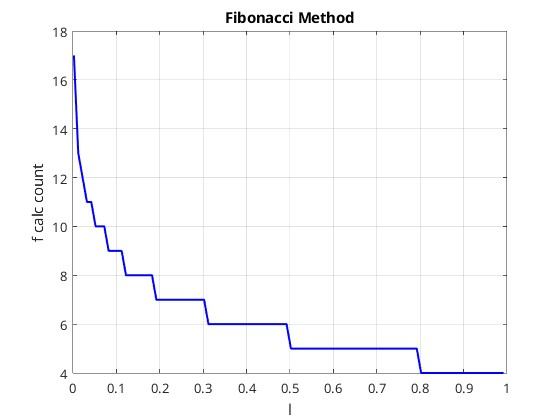
\includegraphics[width=0.5\textwidth]{media/fibonaccif3} % Image file without extension
    \caption{Συνάρτηση $f_3$}
\end{figure}
\subsection{Άκρα του διαστήματος αναζήτησης συναρτήσει του δείκτη επαναλήψεων}
Συνάρτηση $f_1$:
\begin{figure}[H] % h for 'here', you can also use t (top), b (bottom), or p (page)
    \centering
    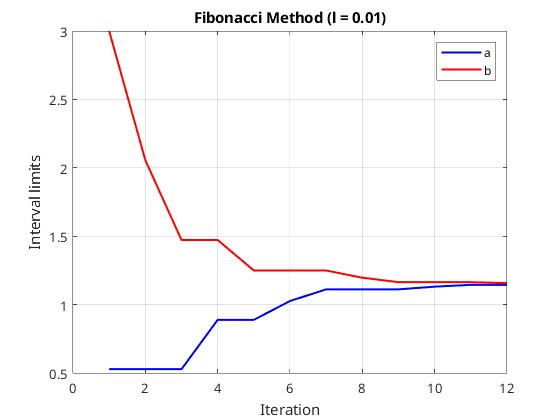
\includegraphics[width=0.5\textwidth]{media/fibonaccif1_001} % Image file without extension
    \caption{Συνάρτηση $f_1$}
\end{figure}
\begin{figure}[H] % h for 'here', you can also use t (top), b (bottom), or p (page)
    \centering
    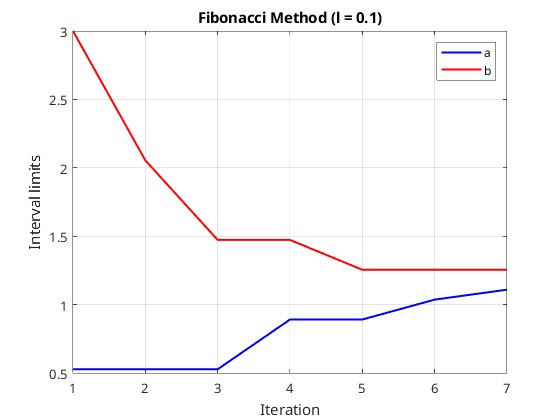
\includegraphics[width=0.5\textwidth]{media/fibonaccif1_01} % Image file without extension
    \caption{Συνάρτηση $f_1$}
\end{figure}
\begin{figure}[H] % h for 'here', you can also use t (top), b (bottom), or p (page)
    \centering
    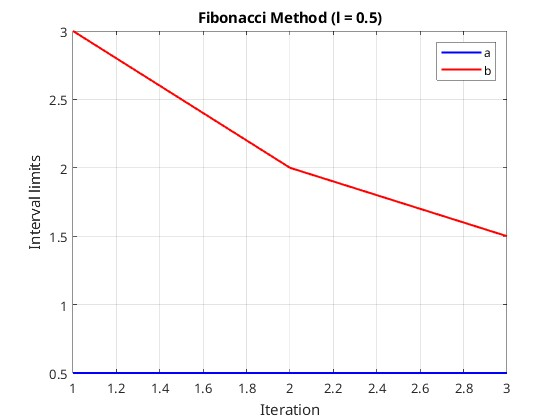
\includegraphics[width=0.5\textwidth]{media/fibonaccif1_05} % Image file without extension
    \caption{Συνάρτηση $f_1$}
\end{figure}

Συνάρτηση $f_2$:
\begin{figure}[H] % h for 'here', you can also use t (top), b (bottom), or p (page)
    \centering
    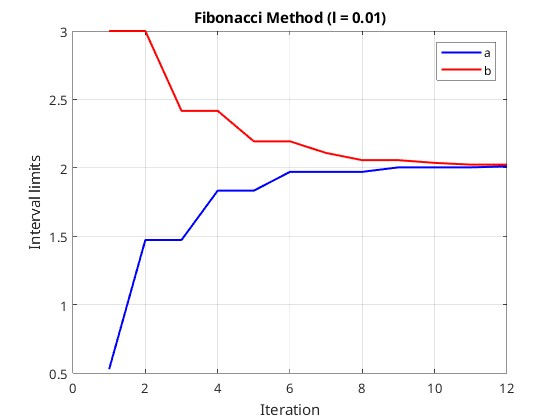
\includegraphics[width=0.5\textwidth]{media/fibonaccif2_001} % Image file without extension
    \caption{Συνάρτηση $f_2$}
\end{figure}
\begin{figure}[H] % h for 'here', you can also use t (top), b (bottom), or p (page)
    \centering
    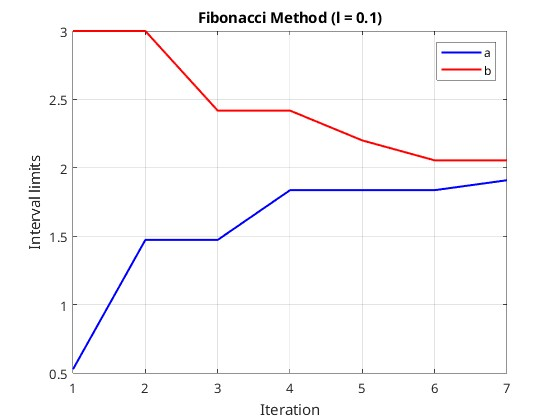
\includegraphics[width=0.5\textwidth]{media/fibonaccif2_01} % Image file without extension
    \caption{Συνάρτηση $f_2$}
\end{figure}
\begin{figure}[H] % h for 'here', you can also use t (top), b (bottom), or p (page)
    \centering
    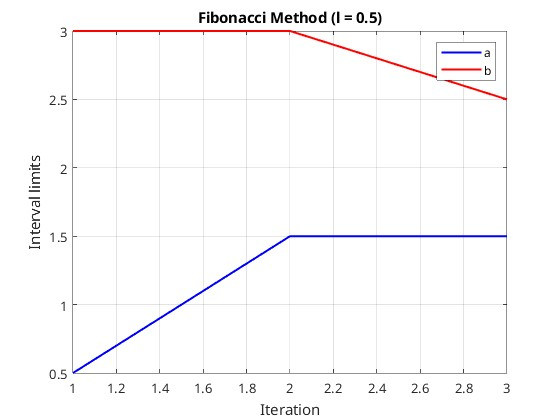
\includegraphics[width=0.5\textwidth]{media/fibonaccif2_05} % Image file without extension
    \caption{Συνάρτηση $f_2$}
\end{figure}

Συνάρτηση $f_3$:
\begin{figure}[H] % h for 'here', you can also use t (top), b (bottom), or p (page)
    \centering
    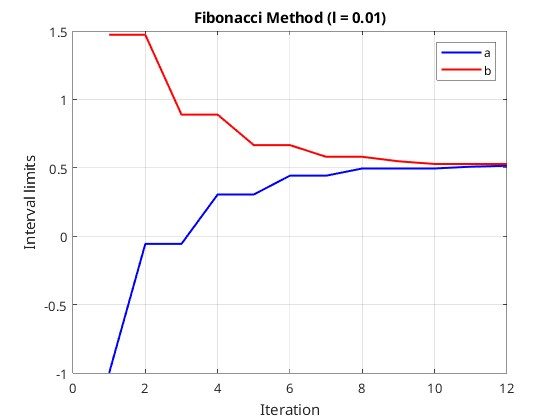
\includegraphics[width=0.5\textwidth]{media/fibonaccif3_001} % Image file without extension
    \caption{Συνάρτηση $f_3$}
\end{figure}
\begin{figure}[H] % h for 'here', you can also use t (top), b (bottom), or p (page)
    \centering
    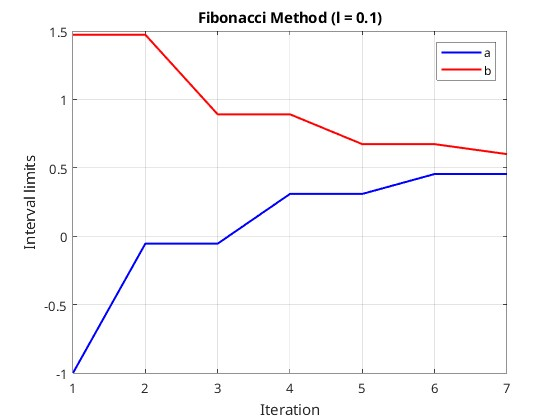
\includegraphics[width=0.5\textwidth]{media/fibonaccif3_01} % Image file without extension
    \caption{Συνάρτηση $f_3$}
\end{figure}
\begin{figure}[H] % h for 'here', you can also use t (top), b (bottom), or p (page)
    \centering
    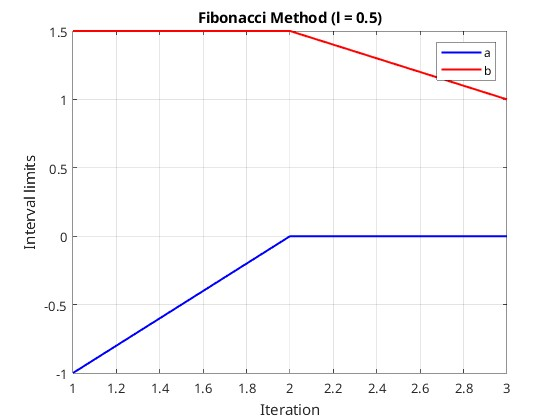
\includegraphics[width=0.5\textwidth]{media/fibonaccif3_05} % Image file without extension
    \caption{Συνάρτηση $f_3$}
\end{figure}

% Dichotomy 2
\chapter{Problem 4}
\section{Prompt}
\subsection Θέμα 4
Επαναλάβετε το Θέμα 2, χρησιμοποιώντας τη μέθοδο της Διχοτόμου με χρήση παραγώγου.
\section{Solution}
\subsection{Κατανόηση Αλγορίθμου}
Ο αλγόριθμος της διχοτόμου (με παραγώγιση) διαφοροποιείται από τον απλό μόνο στο κομμάτι 
επιλογής χωρίου αναζήτησης. Εδώ υπολογίζουμε την παράγωγο της συνάρτησης στο σημείο
διχοτόμησης και ανάλογα με το αν είναι θετική ή αρνητική επιλέγω το αριστερό ή το δεξί
διάστημα ως νέο διάστημα αναζήτησης.  
\subsection{Βήματα Αλγορίθμου}
Όμοια με τον αλγόριθμο της διχοτόμου.
\subsection{Υπολογισμοί αντικειμενικής συνάρτησης συναρτήσει του $l$}

\begin{figure}[H] % h for 'here', you can also use t (top), b (bottom), or p (page)
    \centering
    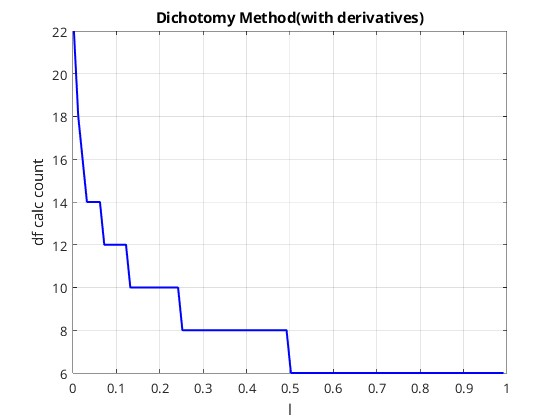
\includegraphics[width=0.5\textwidth]{media/dichotomy2f1_1} % Image file without extension
    \caption{Συνάρτηση $f_1$}
\end{figure}

\begin{figure}[H] % h for 'here', you can also use t (top), b (bottom), or p (page)
    \centering
    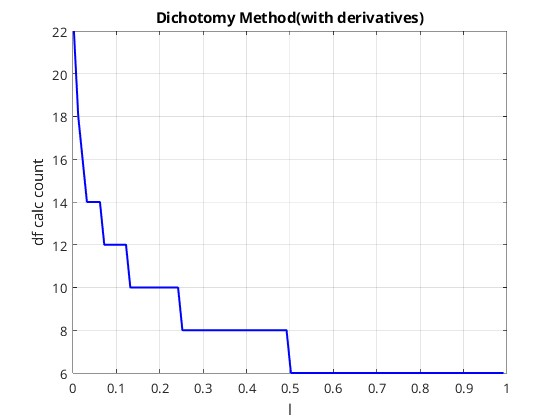
\includegraphics[width=0.5\textwidth]{media/dichotomy2f2_1} % Image file without extension
    \caption{Συνάρτηση $f_2$}
\end{figure}

\begin{figure}[H] % h for 'here', you can also use t (top), b (bottom), or p (page)
    \centering
    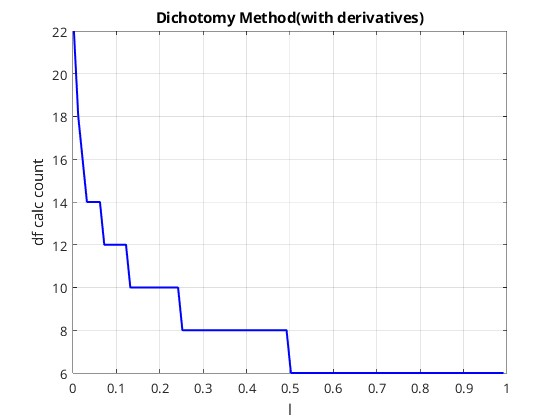
\includegraphics[width=0.5\textwidth]{media/dichotomy2f3_1} % Image file without extension
    \caption{Συνάρτηση $f_3$}
\end{figure}

\subsection{Άκρα του διαστήματος αναζήτησης συναρτήσει του δείκτη επαναλήψεων}
Συνάρτηση $f_1$:
\begin{figure}[H] % h for 'here', you can also use t (top), b (bottom), or p (page)
    \centering
    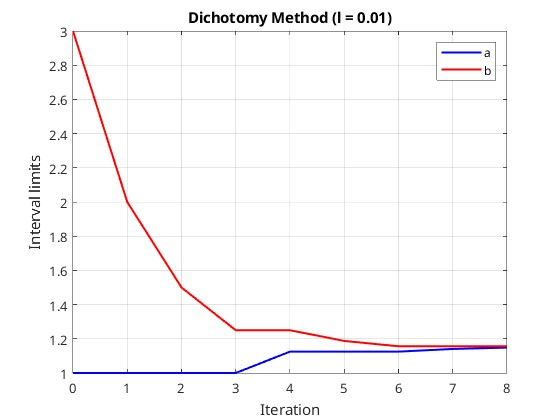
\includegraphics[width=0.5\textwidth]{media/dichotomy2f1_2001} % Image file without extension
    \caption{Συνάρτηση $f_1$}
\end{figure}
\begin{figure}[H] % h for 'here', you can also use t (top), b (bottom), or p (page)
    \centering
    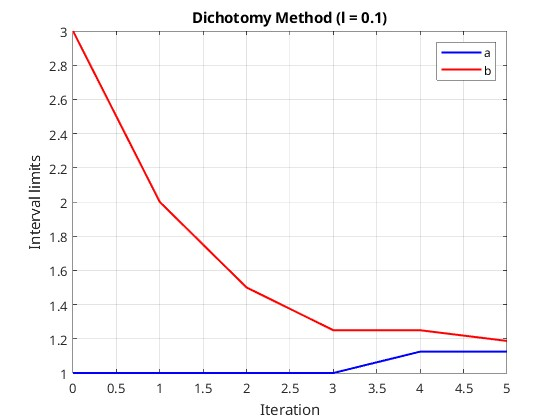
\includegraphics[width=0.5\textwidth]{media/dichotomy2f1_201} % Image file without extension
    \caption{Συνάρτηση $f_1$}
\end{figure}
\begin{figure}[H] % h for 'here', you can also use t (top), b (bottom), or p (page)
    \centering
    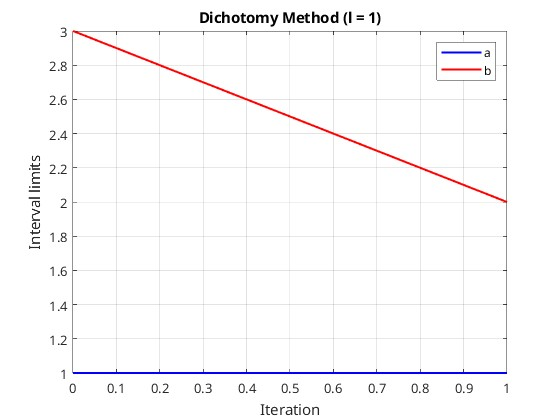
\includegraphics[width=0.5\textwidth]{media/dichotomy2f1_21} % Image file without extension
    \caption{Συνάρτηση $f_1$}
\end{figure}

Συνάρτηση $f_2$:
\begin{figure}[H] % h for 'here', you can also use t (top), b (bottom), or p (page)
    \centering
    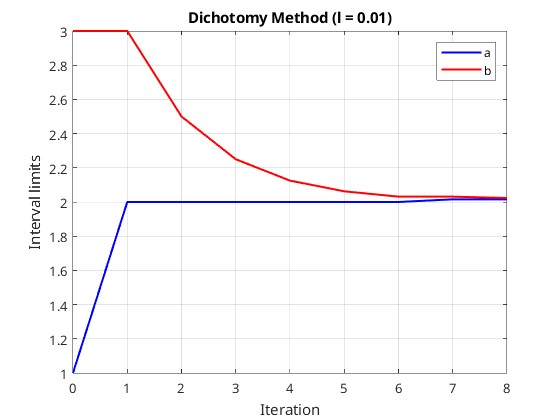
\includegraphics[width=0.5\textwidth]{media/dichotomy2f2_2001} % Image file without extension
    \caption{Συνάρτηση $f_2$}
\end{figure}
\begin{figure}[H] % h for 'here', you can also use t (top), b (bottom), or p (page)
    \centering
    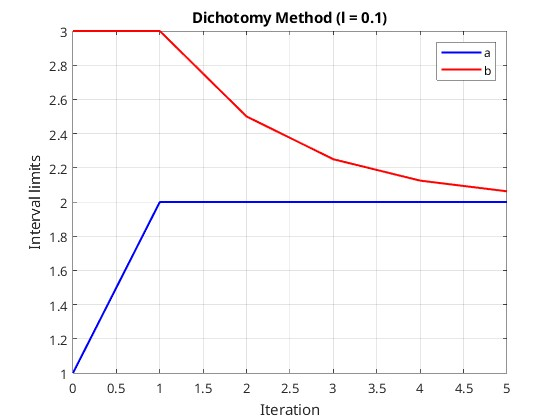
\includegraphics[width=0.5\textwidth]{media/dichotomy2f2_201} % Image file without extension
    \caption{Συνάρτηση $f_2$}
\end{figure}
\begin{figure}[H] % h for 'here', you can also use t (top), b (bottom), or p (page)
    \centering
    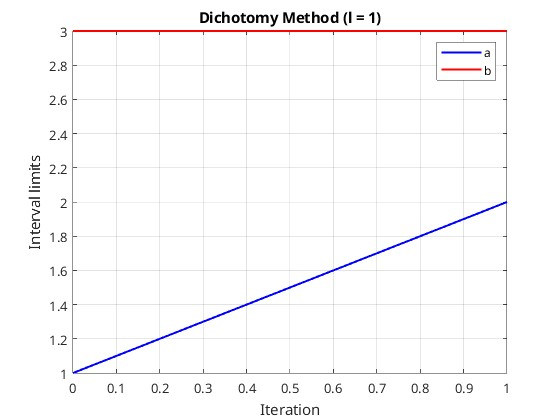
\includegraphics[width=0.5\textwidth]{media/dichotomy2f2_21} % Image file without extension
    \caption{Συνάρτηση $f_2$}
\end{figure}

Συνάρτηση $f_3$:
\begin{figure}[H] % h for 'here', you can also use t (top), b (bottom), or p (page)
    \centering
    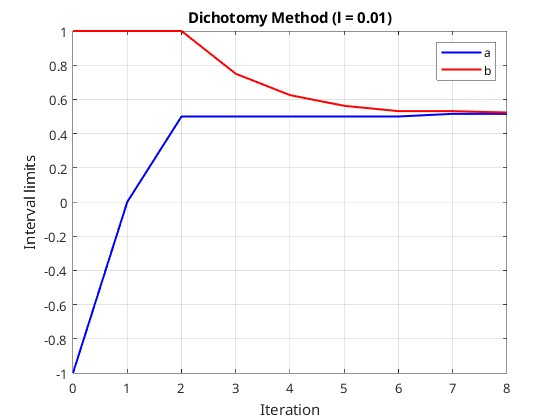
\includegraphics[width=0.5\textwidth]{media/dichotomy2f3_2001} % Image file without extension
    \caption{Συνάρτηση $f_3$}
\end{figure}
\begin{figure}[H] % h for 'here', you can also use t (top), b (bottom), or p (page)
    \centering
    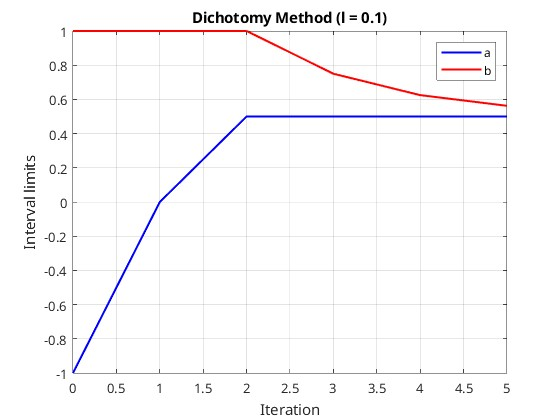
\includegraphics[width=0.5\textwidth]{media/dichotomy2f3_201} % Image file without extension
    \caption{Συνάρτηση $f_3$}
\end{figure}
\begin{figure}[H] % h for 'here', you can also use t (top), b (bottom), or p (page)
    \centering
    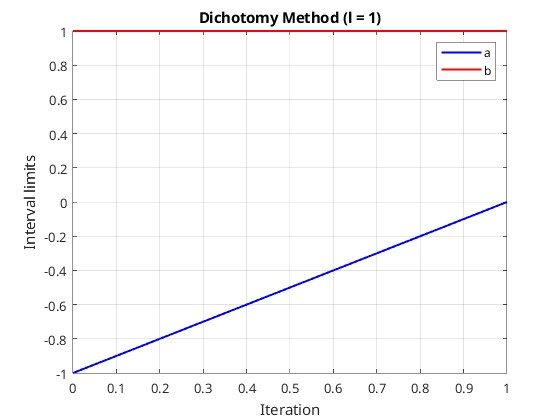
\includegraphics[width=0.5\textwidth]{media/dichotomy2f3_21} % Image file without extension
    \caption{Συνάρτηση $f_3$}
\end{figure}

% Comparison
\chapter{Analysis}
\section{Comparison of the methods}
Πλεονεκτήματα - Μειωνεκτήματα κάθε μεθόδου
\section{Comments}
Τα διαγράμματα του πλήθους υπολογισμών των συναρτήσεων ως προς το $l$ για την ίδια συνάρτηση είναι 
ίδια, όποιον από τους αλγορίθμους και αν εξετάσουμε.

Η ελάττωση του $l$ μας δίνει μεγαλύτερη ακρίβεια στους υπολογισμούς μας, καθώς όταν παίρνει μεγάλες τιμές
ο αλγόριθμός τερματίζει πρόωρα πριν προχωρήσουμε σε πιο μικρά και ακριβή διαστήματα. 



% Bibliography
\nocite{*} % Include all references in the bibliography, even if they are not cited in the report
\bibliographystyle{plain}
\renewcommand{\bibname}{Bibliography}
\bibliography{references/references} % We have to include the references somewhere in the report for them to show here if we don't use (\nocite{*})
\addcontentsline{toc}{chapter}{\bibname}

% End of the document
\end{document}